\section{Test de Shapiro-Wilk}
(Este test es más potente que el de Kolmogorov-Smirnov)

Mide como de bien se ajustan los datos a una distribución normal esperada. Se basa en combinación lineal de estadísticos ordenados. %Esto lo ha añadido en clase

\[
    W=\frac{\left(\sum_{i=1}^{n} a_i \cdot X_{(i)}\right)^2}{\sum_{i=1}^{n}(x_i-\overline{X})^2}
\]

\noindent donde

\begin{itemize}
    \item $X_{(i)}$ es el estadístico de orden \textit{i-ésimo}.
    \item $a_i$ son los coeficientes calculados a partir de los cuartiles esperados de una distribución normal estandar. 
\end{itemize}

\[
    (a_1,a_2,\dots,a_n)=\frac{m^T\cdot v^{-1}}{\sqrt{m^T \cdot V^{-1} \cdot V^{-1} \cdot m}}
\]

\noindent tal que

\begin{itemize}
    \item m=($m_{(1)},\dots,m_{(n)}$)
    \item V es la matriz de las covarianzas de $m_{(i)}$
\end{itemize}

El numerador nos indica como de bien se alinean los datos con la normalidad esperada. Si los datos son normales, el numerador será grande.

\begin{figure}[h!]
    \centering
    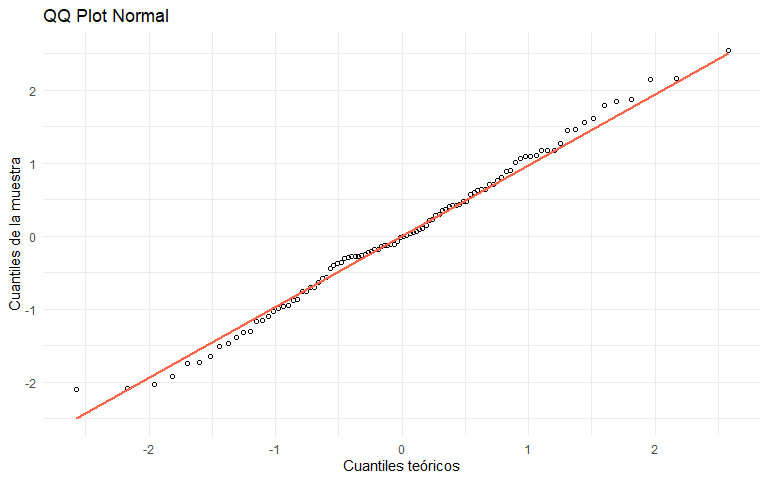
\includegraphics[width=\textwidth]{assets/QQplot.png}
    \caption{Visualización del QQ plot entre una distribución normal y la muestra}
    \label{fig:qqplot_normal}
\end{figure}